\section{Introdução}
Nesta secção é apresentado o trabalho e desenvolvimento dos projetos realizados durante o estágio e á semelhança do capítulo anterior cada projeto será desenvolvido num subcapitulo dedicado.

\section{Coletor de Dados - Nidus} 
\par



\section {NB-Iot \& Digi Xbee 3 }
\par
O desenvolvimento do projeto NB-Iot \& Digi Xbee 3  é composto por 4 fases, 3 das quais desenvolvidas durante este estágio. A fase não desenvolvida durante o estágio refere-se ao desenho e produção do hardware e a parte do software referente á leitura de sensores (comunicação entre hardware desenvolvido e software). As fases realizadas durante o estágio são a implementação do envio do pacote definido com os mecanismos de proteção e segurança, sincronismo dos tempos de leitura e envio e testes ao sistema.

\subsection {Envio de dados para o portal}

\par Como foi indicado no Capítulo \ref{nbiot} a estrutura de pacote a enviar é similar ao do outro produto desenvolvido pela captemp. Este pacote é enviado através de um pacote UDP para o portal que posteiormente confirma a receção na camada de aplicação. O tamanho máximo definido para este pacote é de 1000 bytes.
A estrutura criada pela captemp segue o formato apresentado na figura \ref{packet}.
\par No Primeiro cabeçalho é possivel obter os dados do equipamento que fez o envio tais como a data de envio, o IMEI, a versão do mesmo e o CRC do pacote para confirmar a integridade do mesmo. No restante do pacote são adicionados vários sub pacotes seguindo a estrutura apresentada na figura \ref {packet}, o primeiro byte indica o tipo de dados se é envio o valor de um sensor uma configuraçao do equipamento por exemplo a operadora, o byte seguinte fornece o número de bytes dos dados e posterioremente segundo o número de bytes é dado o valor no exemplo indicado da operadora pode ser a string "ALTICE".

 \begin{figure}[ht]
\centering
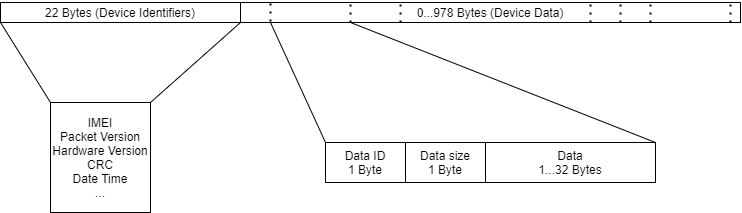
\includegraphics[width=0.95\textwidth]{images/packetnb.png}
\caption{Estrutura do Pacote NB-IOT}\label{packet}
\end{figure}

\subsection {Gestão de memória}

\par O principal motivo da desistencia da utilização deste equipamento como o equipamento principal da Captemp para o NB-iot é a incorreta gestão de memória do MicroPython. Segundo a documentação quando uma variável já não é acessivel pelo código esta é removida pelo \textit{Garbage Collector} mas o espaço de memória  ocupado fica disponivel mas não é mais usado pelo MicroPython e este aloca no final ao invés de procurar o primeiro espaço disponivel. No esquema apresentado na figura \ref{memo} é apresentado o comportamento da memória com a gestão nativa do MicroPython, com o decorrer do tempo a memória fica totalmente alocada não permitindo ao equipamento guardar novas leituras nem enviar para o portal.


 \begin{figure}[ht]
\centering
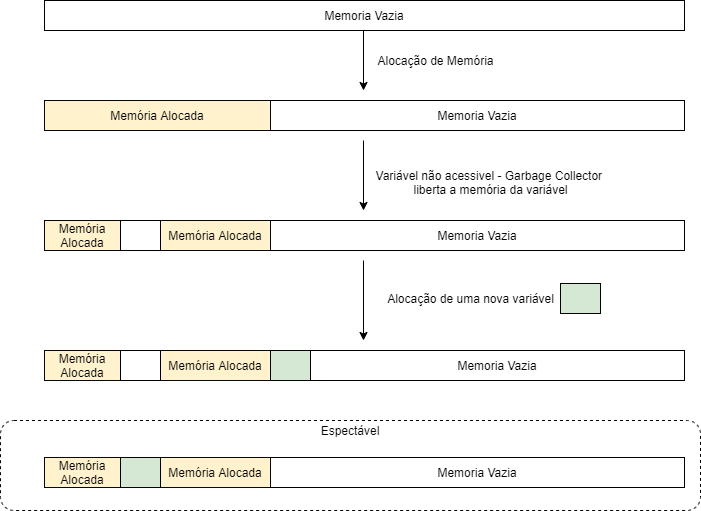
\includegraphics[width=0.95\textwidth]{images/memo.png}
\caption{Comportamento da gestão de Memória}\label{memo}
\end{figure}



\subsubsection {Diminuição da alocação de memória}

\par A modo de resolver a incorreta gestão de memória é necessário diminuir a alocação de novas variáveis. Para tal todo o código do programa visa a possuir todas as constantes e variáveis em variaveis globais as quais nunca são eliminadas e criadas apenas alteram o seu valor. Os dois pontos criticos identificados são o array circular com as leituras dos sensores e a criação do pacote de envio para o portal Cloud.
\par Na criação do pacote todos os cabeçallhos fixos são alocados em constantes globais que não vem o seu valor alterado não afetando a memória e os valores que podem ser alterados são guardados em buffers globais criados no inicio e tem o seu tamanho estático. Como o módulo utilizado não possui suporte para multrithread não existe nunhum problema de sincronismo ao utilizar as variáveis e os buffers globais. Ao recolher um dado de modo a enviar para o portal, como por exemplo a operadora, este tem de ser alocado num buffer que depois é enviado pela rede para o servidor. Este buffer de bytes com o tamanho fixo do máximo do pacote de envio é utilizado para fazer a contatenação dos vários campos antes de enviar. Caso se pretenda adicionar valores a enviar é consultada a ultima posiçao ocupada, encontrada numa váriavel separada e é alterado os bytes das posições seguintes para o bytes do valor não alocando espaço para continuar o array.
\par Supondo que o buffer tem já preenchidos 300 bytes dos 1000, ao pretender adicionar o pacote da operadora, é copiado para a posição 301 o byte correspondente áo DATA ID do operador, no byte seguinte é colocado o tamanho de bytes que a operadora ocupa ("ALTICE"= 6 Bytes), e nos seguintes 6 bytes é colocada a string.
\par No exemplo acima elucidado todas a variável DATA ID é estática e definida no inicio do código, o tamanho foi previamente guardado numa variavel auxiliar de tamanho fixo, e a operadora é soilicatado a funções nativas do MicroPtyhon  e guardado num buffer de tamanho fixo. Após a definição apenas são efetuadas copias de bytes entre variaveis e buffers não afetando a alocação de memória. No código seguinte é exempleficado  a operação anteriormente apresentada. Neste caso de modo a simplificar é apresentado um buffer do tamanho da operadora, no projeto foram criados buffers do tamanho 1,2,4,10,16,32 bytes consoante os valores mais comuns, no caso particular de um valor que possa ter por exemplo 20 bytes este é guardado no buffer de 32 e no momento da gravacao apenas são copiados os 20 primeiros bytes.

	
\begin{verbatim}
	c=bytearray(1000) # Packet Array
	clean=bytearray(1000) # Empty Packet Array 

	#BUFFERs

	cmd6=bytes(6)
	cmdID=bytes(1)
	cmdLEN=bytes(1)

	#DATA IDs
	c0=bytes([0x01])
	
	(...)	

	cmdID = c0 #  DATA ID
	cmdLEN = (6).to_bytes(1, 'little') # Data Size
	cmd6 = (oper).to_bytes(2, 'little') # Data
	byteschange(c, 300, 301, cmdID) # Copy to packet array 
	byteschange(c, 301, 302, cmdLEN)  # Copy to packet array 
	byteschange(c, 302, 308, cmd6)  # Copy to packet array 
 \end{verbatim}

\par Ao copiar valores de entre buffers e não alocando espaço para o array crescer é necessário um maior controlo nos tamanhos das variáveis de modo a não copiar valores de buffers vazios ou posições enexistentes. A versão do MicroPython disponibilizada pela Digi não incorpora a biblioteca que faz a gestão de arrays limitando não possibilitando a copia direta de arrays para outros arrays indicando apenas a posição inicial. Para tal a função byteschange definida previamente no código, simula essa operação onde apenas indicamos o buffer de destino, a posiçao inicial, a final e a origem da cópia. Esta função é responsável por verificar se os tamanhos são possiveis de copiar e copia posição a posição (byte a byte no caso apresentado) para as posiçoes entre os valores indicados. No fim do pacote ser enviado é possivel limpar o buffer chamando a mesma função indicando como origem da copia o buffer clean, um buffer constante do mesmo tamanho mas com os bytes todos vazios. Todos os buffers utilizados ao longo do projeto tem um semelhante em tamanho mas completamente vazio. Deste modo é possivel utilizar sempre os mesmos buffers e não existir a necessidade de alocar buffers ao longo do programa.

\subsubsection {Gestão da memória durante leituras}

\par À semelhança do buffer onde é criado o pacote enviado para o portal, as leituras são um dos pontos criticos referente á alocação de memória. Para tal á semenlhança do pacote de envio, é inicializado no inicio do programa, um array de tamanho fixo e com cada posição com um array do tamanho máximo de cada leitura. Ao adicionar uma nova leitura são colocados nos buffers intermédios todos os dados e são copiados para a posição seguinte á ultima posiçã ocupada. Caso a ultima posição ocupada corresponda à ultima do array, é adicionado sobre a primeira posição, criando assim o array circular.
\par Todas as operações para adicionar uma leitura ao array ou remover são efetuadas com a função byteschange de  copiando o buffer temporátio com a leitura ou o vazio respetivamente. Na figura \ref{circbuf} é apresentado o esquema do array circular com as leituras. Como array é definido inicialmente e o utilizador pode alterar as sondas enquanto o equipamento está em funcionamento é sempre alocado para cada leitura o máximo de sensores garantindo que caso o utilizador adicione um sensor não seja necessário expandir o tamanho da posiçao no array causando os problemas de memoria já identificados. Para eliminar a posição é decrementado a posição currente do array e por proteção de modo a posteriormente não acedermos a dados que possam la existir, como por exemplo numa leitura antiga com 6 sensores e nova com 3 sensores os ultimos 3 sensores da leitura antiga ainda estavam associados apesar de no cabeçalho da leitura indicar que eram apenas 3. Zerando o buffer garantimos que por algum lapso ocorra leituras erradas da zona do buffer a mesma nao irá afetar nenhuma leitura.


 \begin{figure}[ht]
\centering
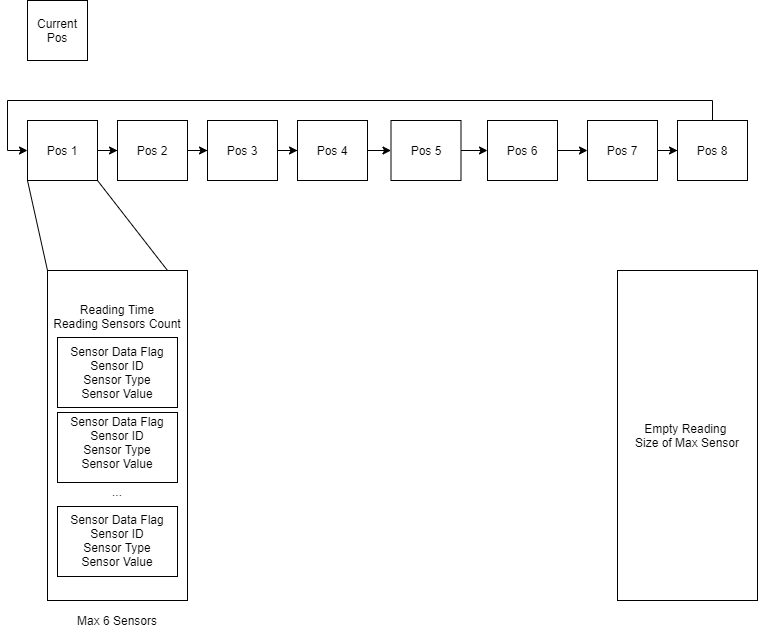
\includegraphics[width=0.85\textwidth]{images/circbuf.png}
\caption{Array Circular com leituras}\label{circbuf}
\end{figure}

\subsection {Sincronismo de Leitura e Envio} 

\par À semelhança dos restantes produtos produzidos pela captemp existe sempre sincronismo de leituras entre os equipamentos. Para tal além de cada equipamento possuir um relógio interno (RTC), é necesário fazer o sincronismo na primeira leitura, ou seja caso esteja programado para fazer a leitura a cada 5 minutos, existe uma diferença caso o mesmo seja ligado ás 00:00 e fazer as leituras respetivamente às 00:05, 00:10,00:15,00:20 , mas caso seja ligado por exemplo às 00:12, faz leituras às 00:17,00:00:22 e por diante não existindo um sincronismo entre os vários equipamentos dos clientes.
\par Para tal o equipamento no momento inicial do arranque verifica qual o intervalo de leitura e de envio, e verifica caso fosse ligado pelas 00:00 qual seria a proxima leitura ao momento atual, neste momento o equipamento não entra em modo de poupança de energia durante os 5 minutos até á leitura e apenas o tempo restante até ao valor caso fosse ligado pelas 00:00, no momento da leitura o equipamento já entra em modo de poupança de energia durante o tempo definido (Ex:5 minutos). Este método é igualmente aplicado ao intervalo de envio. Aquando do envio é enviado na resposta proveniente do servidor o \textit{Timestamp} do servidor de modo a sincronizar o tempo de todos os equipamentos e configurar nos novos equipamentos que sejam ligados e ainda possuam o valor default do RTC, no caso do escolhido no projeto 1 de Janeiro de 2000.
\par Caso o equipamento possuir uma data inferior á estipulada de 1 de Janeiro de 2019, o mesmo não faz leituras, esperando pelo intervalo de envio para enviar um pacote apenas com os campos fixos e sem leituras de modo a obter a resposta com o \textit{Timestamp} do servidor para iniciar as leituras.


\subsection {Encriptação dos dados}

\par De modo a proteger os dados na rede todo o pacote é encriptado con recurso á biblioteca MicroPython-AES disponibilizada online !!!!!!!!!!!!!!! colocar link do github. !!!!!!!!!!!!!!!!!!!!!!!. De modo a exta biblioteca desenvolvida para o MicroPython Base e não para a versão disponibilizada nos módulos DIGI, é necessário reconstruir a biblioteca para nao utilizar a biblioteca dos arrays  indisponivel nesta versão e fazer a alteração para a função byteschange ou aquando da necessidade de acrescentar dados no array colocar posição por posição. 


\begin{verbatim}
...
for offset in range(0, len(data), block_size):
    block = data[offset:offset + block_size]
    block_func(block)
    data[offset:offset + block_size] = block # ERROR 
    #['array' object does not support item assignment]
...

...
for offset in range(0, len(data), block_size):
    block = data[offset:offset + block_size]
    block_func(block)
    # Solution ['array' object does not support item assignment]
    for i in range(block_size)
        data[offset+i]= block[i]
...
 \end{verbatim}

\section {Kea Tracker}

\par De modo a substituir um produto descontinuado e apresentar novas soluções aos clientes, irão ser utilizadas beacons da Ruuvi Tag para



\section {dot.Tracker}
\par
A pedido de um cliente, foi proposto o desenvolvimento de uma plataforma WEB para fazer a monitorização de pessoas e objetos em tempo real. O projeto passou por várias  etapas das quais destacam-se a análise dos requesitos do cliente, anáilise de tecnologias disponiveis, análise de soluções existentes já em comercialização, o desenvolvimento do portal Web, desenvolvimento do Back-End, e testes ao sistema. Apesar do projeto ser apenas desenvolvido por um elemento, mas devido á maior complexidade e duração do mesmo foi adotada a metodlogia SCRUM com entregas/apresentações ao cliente para obter o feed-back do trabalho desenvolvido e assim poder alterar alguns dos requesitos solicitados.
\par O Cliente indicou que devia ter atualizações dos mapas em tempo real, alertas enviados para o cliente WEB caso este esteja online e por email.
É assim possivel definir a tabela, apresentada na tabela \ref{tab1} com os requisitos da solução e a sua importância no desenvolvimento.

\begin{table}[htb]
\centering
\caption{Requesitos da Solução}\label{tab1}
\begin{tabular}{|p{3cm}|p{8cm}|p{2cm}|}\hline
Requesito&Descrição&Importância (1-10)\\\hline

Portal Cloud (Front-End)&Portal Cloud com mapas em tempo Real& 7\\\hline
Portal Cloud (Back-End) & API REST para integração com o Front-End e recolha dos dados para a localização &9\\\hline
Histórico de posições&Possibilidade de revisualizar no mapa o percurso entre datas&5\\\hline
Alertas Email&Alertas de Email (Exemplo: Entrada e Saída de zonas criadas no mapa)&6\\\hline
Alertas Web&Alertas Informativos no Mapa(Exemplo: Entrada e Saída de zonas criadas no mapa)&2\\\hline
\end{tabular} 
\end{table}

\par
De seguida são apresentados as funcionalidades e objetivos de cada requesito e escolhas selecionadas.

\subsection {Portal Cloud -  Front-End}

\par O Front-end da solução é desenvolvido com recurso á Framework Vue, tornando a solução numa solução Single-Page Aplication. A adoção da Framework é baseada na necessidade de possuir fluidez na navegação entre páginas e igualmente nos mapas em tempo real minimizando o delay.
\par A plataforma é capaz igualmente de suportar várias \textit{Companies}, significa isto que é possivel criar várias \textit{Companies} e temos os administradores e os utilizadores normais de cada \textit{Company} que apenas tem acesso ás suas definições e equipamentos. Possibilitando fornecer o projeto como uma solução Cloud a váriados clientes no mesmo Servidor, onde cada um apenas possui o acesso ao que pertence à sua \textit{Company}.
No final o utilizador da plataforma deve ser capaz de realizar as seguintes operações:
\par
\begin{itemize}
\item Login na Plataforma para visualizar os dados
\item Vizualizar um mapa com atualizações em tempo real
\item Editar o seu perfil
\item Visualizar a página numa língua á sua escolha
\item Utilizar a plataforma em vários equipamentos PC,Tablet,Smartphone,...
\item Gerir Utilizadores (Administradores)
\item Gerir Equipamentos (Administradores)
\item Gerir Mapas e Zonas (Administradores)
\item Gerir Alertas (Administradores)
\item Iniciar/ Finalizar Missões (Administradores)
\end{itemize}
\par


\subsection{ Portal Cloud - Back-end}

\par O Back-End é responsável por fornecer uma API REST ao Front-end para o mesmo obter os dados da base de dados. É igualmente responsável por obter os dados proveninentes dos gateways das beacons e calcular as suas posiçoes para apresentar no mapa. 
\par O primeiro problema a identificado no back-end é a necessidade de possuir atualizações em tempo real das posições. O Front-end não é capaz de calcular quando uma beacon comunica com o back-end apesar da mesma enviar o broadcast em tempos regulares, mas tanto a beacon  pode não estar ao alcance do gateway, como a mesma pode apenas estar ao alcance de menos de X(dependendo do algoritmo) gateways impossibilitando a utilização do algoritmo. 
\par Para tal além do serviço web é disponibilizado um servidor de WEB-Sockets para comunicações em tempo real entre o Back-end e o Front-End. Os WEB-Sockets é uma tecnologia que permite aos browsers mais recentes, ter um canal em tempo real com o back-end sem a necessidade de fazer um pedido HTTP, o que acarreta todo o processo do protocolo, como por exemplo o \textit{3-Way Handshake}. No momento da criação do websocket é criado uma ligação TCP a qual não é finalizada até ao fechar do websocket, o que elemina o sobrecarregamento da criação de pedidos e soluciona o problema da comunicação em tempo real para as atualizações dos mapas.
\par Outro problema e solucionar deparado na análise das tecnologias e soluções existentes é a falta de sincronismo da comunicação dos gateways. Supondo um exemplo com 5 gateways e 1 beacon. A beacon ao intervalo de tempo X1 comunica o pacote e apenas 4 gateways recebem o pacote e o enviam para o servidor através de um pedido HTTP. O servidor apesar de ter configurado 5 gateways não é capaz de prever se o 5º gateway irá comunicar a transmissão da beacon, o mesmo pode não estar ao alcance, pode não ter comunicação ao servidor, pode estar desligado ou pode haver algum problema na rede que atrase a chegada do pacote. Igualmente por variados motivos os 4 gateways que enviaram o pacote ao servidor não irão chegar todos em simultaneamente, criando o problema "Já chegaram todos os pacotes? Calculo com os que tenho, ou espero que chegue mais algum pacote?",
\par O primeiro passo para resolver o problema acima citado ao contrário das soluções mais tradicionais não irá ser utilizado um serviço WEB como o APACHE2 ou o NGINX, pois o mesmo não possui nenhum sincronismo entre pedidos e seria necessário armazenar momentaneamente todos os pacotes na base de dados e ter a tabela em constante escrita e leitura, não sendo o mais eficaz no cenário deste projeto. Para tal o serviço web irá ser responsabilidade do NodeJS(módulo express) que irá ter além do serviço WEB o servidor de WEB-Sockets, centralizando assim os dois serviçoes e possibilitando igualmente durante o processamento do pedido HTTP o envio de mensagens através do WEB-Socket. 
\par Na lista apresentada de seguida estão selecionados os pontos principais das funcionalidades do Back-End:

\par
\begin{itemize}
\item API REST para o Front-End (Login+ Dados)
\item API REST para o POST dos Gateways
\item Serviço WEB (express) para disponibilizar o Front-End 
\item Serviço WEB-Sockets 
\item Algoritmo de posicionamento
\item Envio de Alertas
\end{itemize}
\par



\par
